\chapter{Optimisation d'une ressource dans un problème de jobshop}
Cette fois ci, nous allons nous concentrer sur la modélisation d'un problème à base de \emph{jobshop} dans lequel nous étudierons le travail entre deux machines $M_1$ et $M_2$ sur deux pièces $A$ et $B$. Dans un premier temps, nous modéliserons comme dans le chapitre précédent, le GET associé à notre système. Puis nous étudierons chaque marquage initial de notre graphe, selon les ordonnancement possible, afin de déterminer le cycle de temps associé de chacun.

\section{Étude du problème}
%% Ordonnancement 1	:		M2 --> A		B
%%							M1 -->   A - B

%% Ordonnancement 2	:		M2 -->   B - A		NON RESPECT
%%							M1 -->   A - B		NON RESPECT

%% Ordonnancement 3	:		M2 --> 	 A - B
%%							M1 --> 	 B - A

%% Ordonnancement 4	:		M2 --> 	  B	- A
%%							M1 --> B 		A
Le problème de cet exercice peut être décomposé en deux sous problèmes équivalents. Le premier concerne l'ordre dans lequel les pièces $A$ et $B$ peuvent être traités par les machines : $A$ ne peut pas passer sur $M_1$ tant qu'elle n'est pas d'abord passer sur $M_2$. Pour la pièce $B$, elle doit d'abord passer par $M_1$ puis elle va sur $M_2$, comme cela est expliqué dans l'ennoncé. 

Le deuxième problème qui apparait n'en ai pas vraiment un, il s'agit de choisir l'ordonnancement des usinages de pièces. Très naturellement, pour 2 machines et 2 pièces il vient $2\times 2$ possibilité d'ordonnancement qui sont : \begin{enumerate}
\item \label{item:o1}\textbf{Ordonnancement 1} $M_2 \rightarrow A$ puis $M_1 \rightarrow A \rightarrow B$ et  $M_2 \rightarrow B$ 
\item \label{item:o2}\textbf{Ordonnancement 2} $M_2 \rightarrow B \rightarrow A $ parallèle à $M1 \rightarrow A \rightarrow B$
\item \label{item:o3}\textbf{Ordonnancement 3}	$M_2 \rightarrow A \rightarrow B $ parallèle à $M1 \rightarrow B \rightarrow A$
\item \label{item:o4}\textbf{Ordonnancement 4}	$M_1 \rightarrow B$ puis $M_2 \rightarrow A \rightarrow B$ et  $M_1 \rightarrow B$
\end{enumerate}

Pour modéliser notre problème sous forme de GET, nous aurons besoin des évènements qui lient les machines et les pièces entre elles. Nous pouvons obtenir ces informations à partir du tableau donné dans le sujet de TP,  Ces temps d'attentes seront utilisés dans les temps d'attentes des places du GET pour modéliser le temps que met une pièce à être usiné par une machine. L'entrée d'un jeton dans une place signifie le début du traitement d'une pièce par une machine, la fin de traitement est modélisé par la fin de l'attente d'un jeton dans une place. 

Les événements qui lient les machines aux pièces sont donc les les liaisons $A$ entre dans $M_1$, $B$ entre dans $M_1$, $A$ entre dans $M_2$ et $B$ entre dans $M_2$. Nous nous intéressons qu'aux entrés dans les machines car ce sont les événements les plus importants dans un système industriel. En effet les sortie dépendent des temps de traitement et des temps d'entrée : temps de sortie = temps de l'entrée + temps de traitement.

\section{Modélisation des GET et représentation d'état et analyse du cycle associé}

Dans un premier temps, nous avons réalisé le graphe des événements temporisés général(voir figure \ref{fig:get}). Ce graph a 4 transitions (en noir) qui se retrouvent sur les intersections être une pièce et une machine qui est doit usiner la pièce. Elles correspondent, en partant de celle en haut à gauche et dans le sens horaire, à \emph{A entre dans M1}, \emph{B entre dans M1}, \emph{B entre dans M2} et à \emph{A entre dans M2}. 

Les annotations \emph{A}, \emph{B}, \emph{M1} et \emph{M2} ne font pas partis du graph, elles font offices de légendes pour la couleurs des éléments du graph.

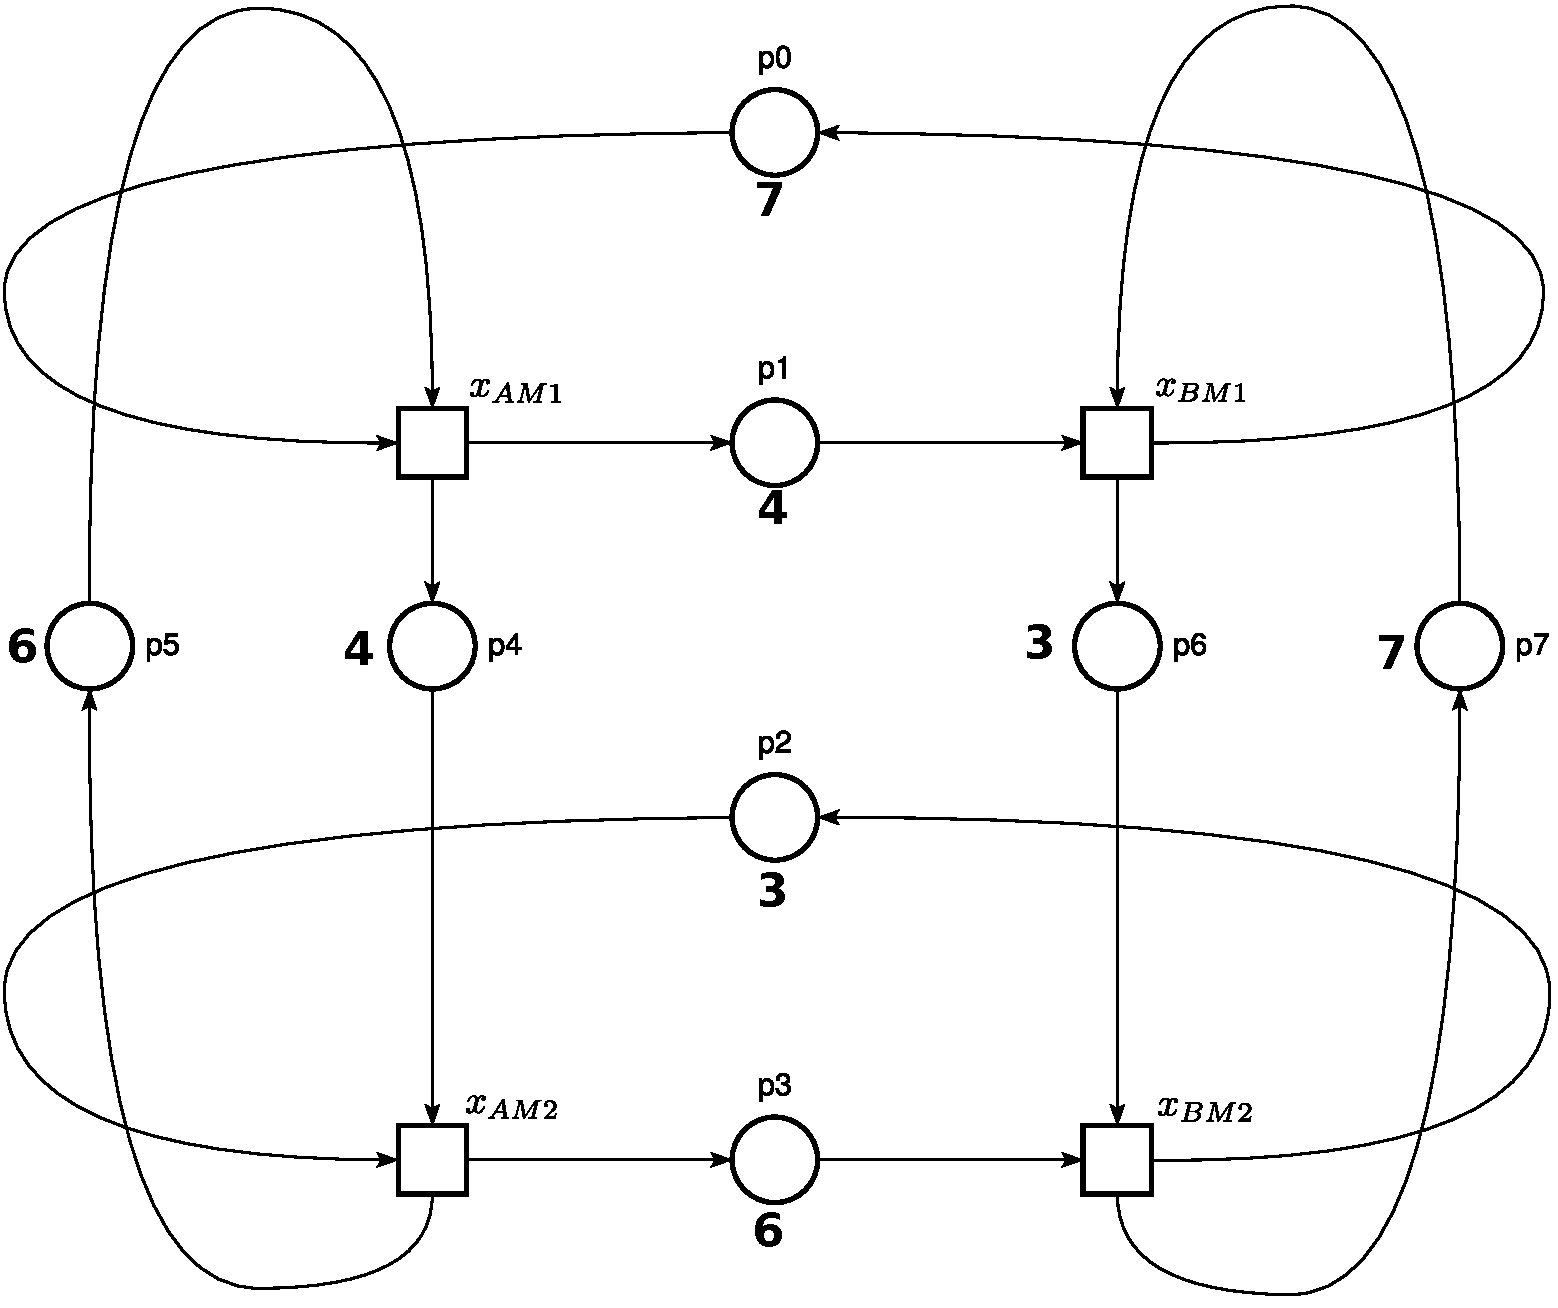
\includegraphics[width = \textwidth]{./II/images/GET.pdf}
\captionof{figure}{\label{fig:get} Graphe des Événements Temporisé du \emph{jobshop}}

\subsection{Ordonnancement 1}
Nous modélisons maintenant le cas du premier ordonnancement possible décrit rapidement en \ref{item:o1}. Dans ce cycle, la pièce $A$ doit d'abord passer sur la machine $M_2$ puis prendre la machine $M_1$. Ensuite c'est au tour de la pièce de prendre les machines $M_1$ puis $M_2$. 

Pour que la pièce $A$ occupe la première utilisation de $M_2$, nous devons placer le marquage initial dans les places $p4$ et $p2$ pour sensibiliser la transition $x_{AM2}$ et ainsi modéliser l'entrer de $A$ dans la machine 2. On souhaite aussi que $A$ utilise la machine 1 avant $B$, donc on empêche la sensibilisation de $x_{BM1}$ en ne mettant pas de jeton dans la place $p1$ mais en plaçant un jeton dans la place $p1$. Pour que la pièce $B$
\begin{figure}[!ht]
\centering
%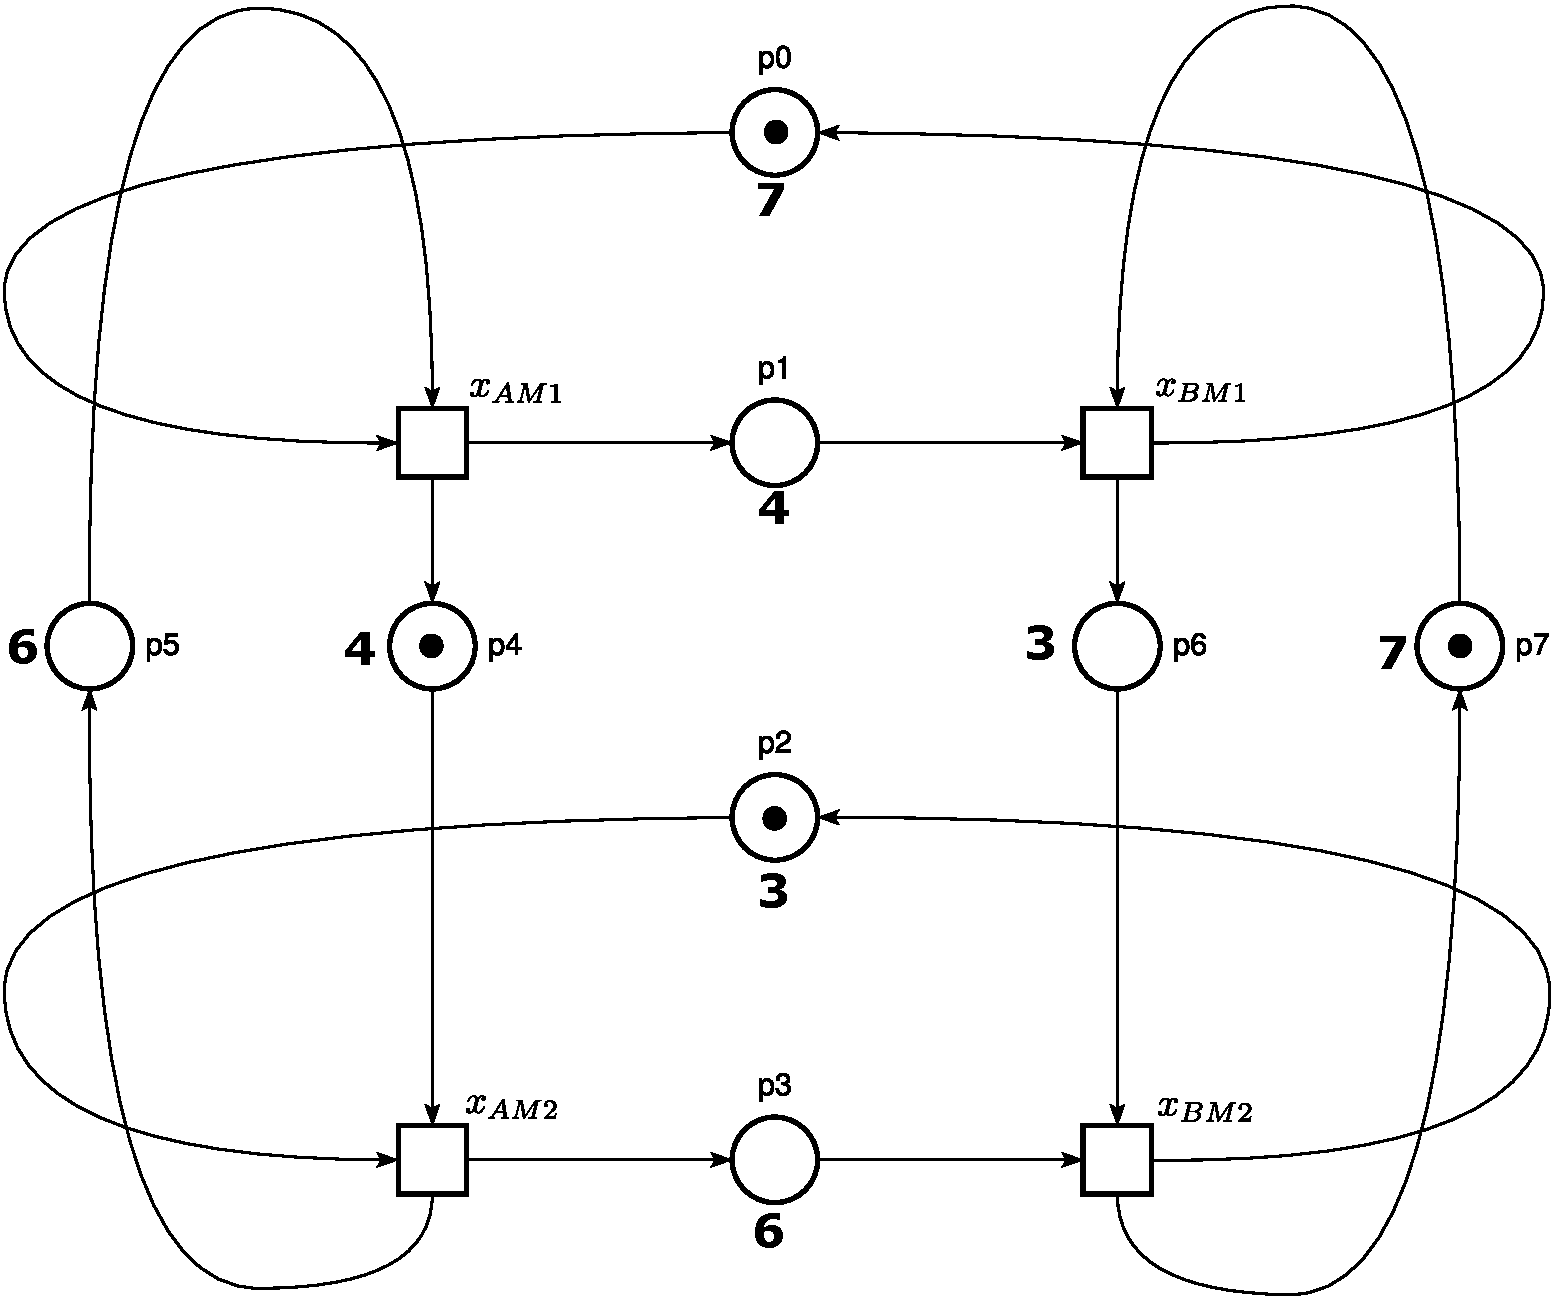
\includegraphics[width = \textwidth]{./II/images/GET_1.pdf}
\caption{\label{fig:get} Graphe des Événements Temporisé de l'ordonnancement 1 (\ref{item:o1})}
\end{figure}

\begin{align*}
\left\lbrace
\begin{array}{lcl}
x_{AM_1}(k)&=& 10x_{AM_1}(k-1) \oplus 9x_{BM_2}(k-1)\oplus 7x_{BM_1}(k-1)\\
x_{AM_2}(k)&=&4x_{AM_1}(k-1) \oplus 3x_{BM_2}(k-1)\\
x_{BM_1}(k)&=& 11x_{BM_1}(k-1) \oplus 14x_{AM_1}(k-1) \oplus 13x_{BM_2}(k-1)\\
x_{BM_2}(k)&=& 20x_{BM_2}(k-1) \oplus 21x_{AM_1}(k-1) \oplus 18x_{BM_1}(k-1)\\
\end{array}
\right.
\end{align*} Pour pouvoir utiliser les analyse qui donne une représentation d'état suivante : 
\begin{align}\label{equ:ordo1}
X(k) = \begin{pmatrix}
x_{AM1}(k) \\ x_{AM2}(k) \\ x_{BM1}(k)\\ x_{BM2}(k)
\end{pmatrix} 
= \begin{pmatrix}
10 & \epsilon & 7 &9\\
4 & \epsilon & \epsilon & 3\\
14 & \epsilon & 11 & 13\\
21 & \epsilon & 18 & 20
\end{pmatrix}X(k-1) = A_1X(k-1)
\end{align}
Pour trouver le temps de cycle, nous proposons d'analyser le ou les valeurs propres de A. Nous obtenons avec ScicosLab et la fonction \emph{karp} le résultat suivant : \begin{eqnarray*}
\lambda(A_1) = 20
\end{eqnarray*}
OBSERVATION NECESSAIRE !!!!!!! %%% TODO
\subsection{Ordonnancement 2}
L'ordonnancement 2 n'est pas réalisable.
\subsection{Ordonnancement 3}
\begin{figure}[!ht]
\centering
%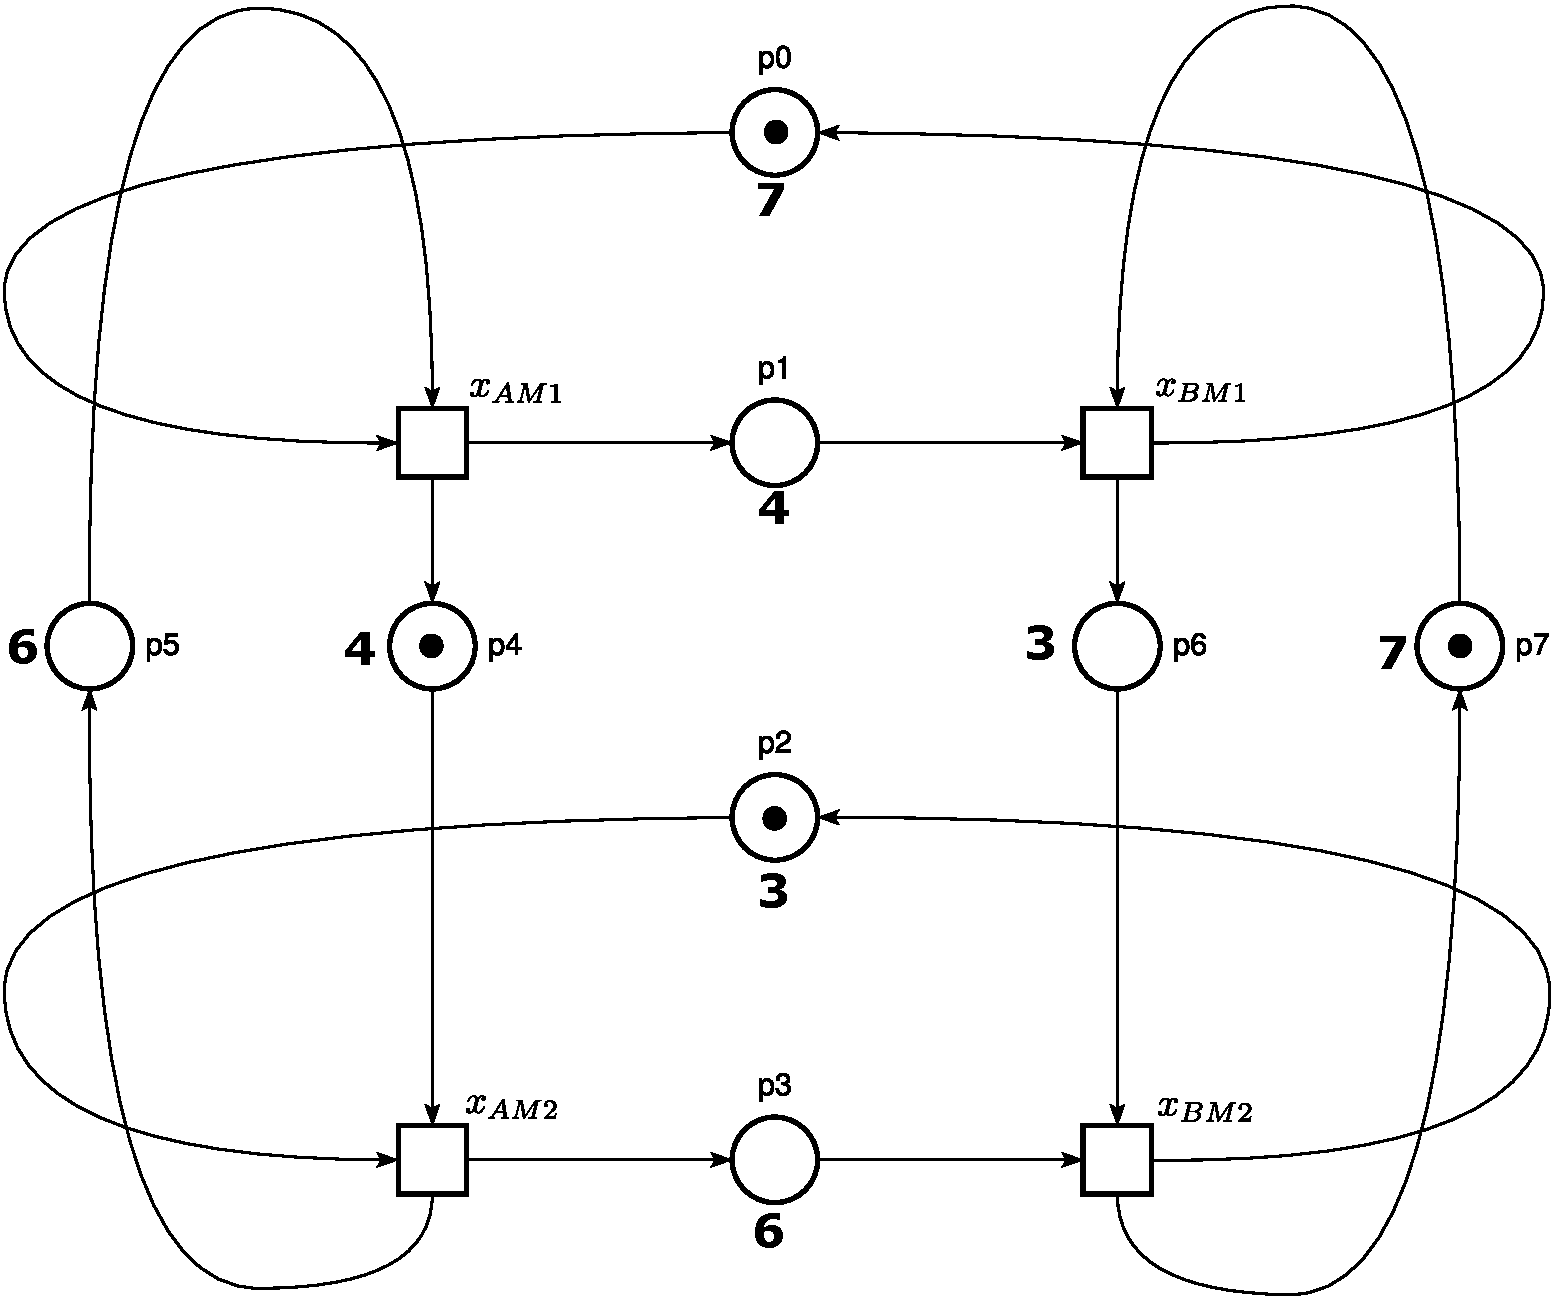
\includegraphics[width = \textwidth]{./II/images/GET_1.pdf}
\caption{\label{fig:get} Graphe des Événements Temporisé de l'ordonnancement 3 (\ref{item:o3})}
\end{figure}
\begin{align*}%\label{equ:ordo3}
\left\lbrace
\begin{array}{lcl}
x_{AM_1}(k)&=& 10x_{AM_1}(k-1) \oplus  9x_{BM_2}(k-1)\\
x_{AM_2}(k)&=&  4x_{AM_1}(k-1) \oplus  3x_{BM_2}(k-1)\\
x_{BM_1}(k)&=&  4x_{AM_1}(k-1) \oplus  3x_{BM_2}(k-1)\\
x_{BM_2}(k)&=& 10x_{BM_2}(k-1) \oplus 11x_{AM_1}(k-1)\\
\end{array}
\right.
\end{align*}
Ce système d'équation du GET peut être représenté sous forme espace d'état avec le même vecteur que d'état que dans \ref{equ:ordo1}. Nous obtenons :
\begin{align}\label{eqn:eeOrdo3}
X(k) = \begin{pmatrix}
10 & \epsilon &\epsilon & 9\\
4 &\epsilon &\epsilon & 3\\
4 &\epsilon &\epsilon & 3\\
11 &\epsilon &\epsilon & 10\\
\end{pmatrix}X(k-1) = A_2X(k-1)
\end{align} 
Comme pour l'ordonnancement précédent, nous calculons la valeurs propres du système pour le temps de cycle : 
\begin{eqnarray*}
\lambda(A_2) = 11  
\end{eqnarray*}

\subsection{Ordonnancement 4}
\begin{figure}[!ht]
\centering
%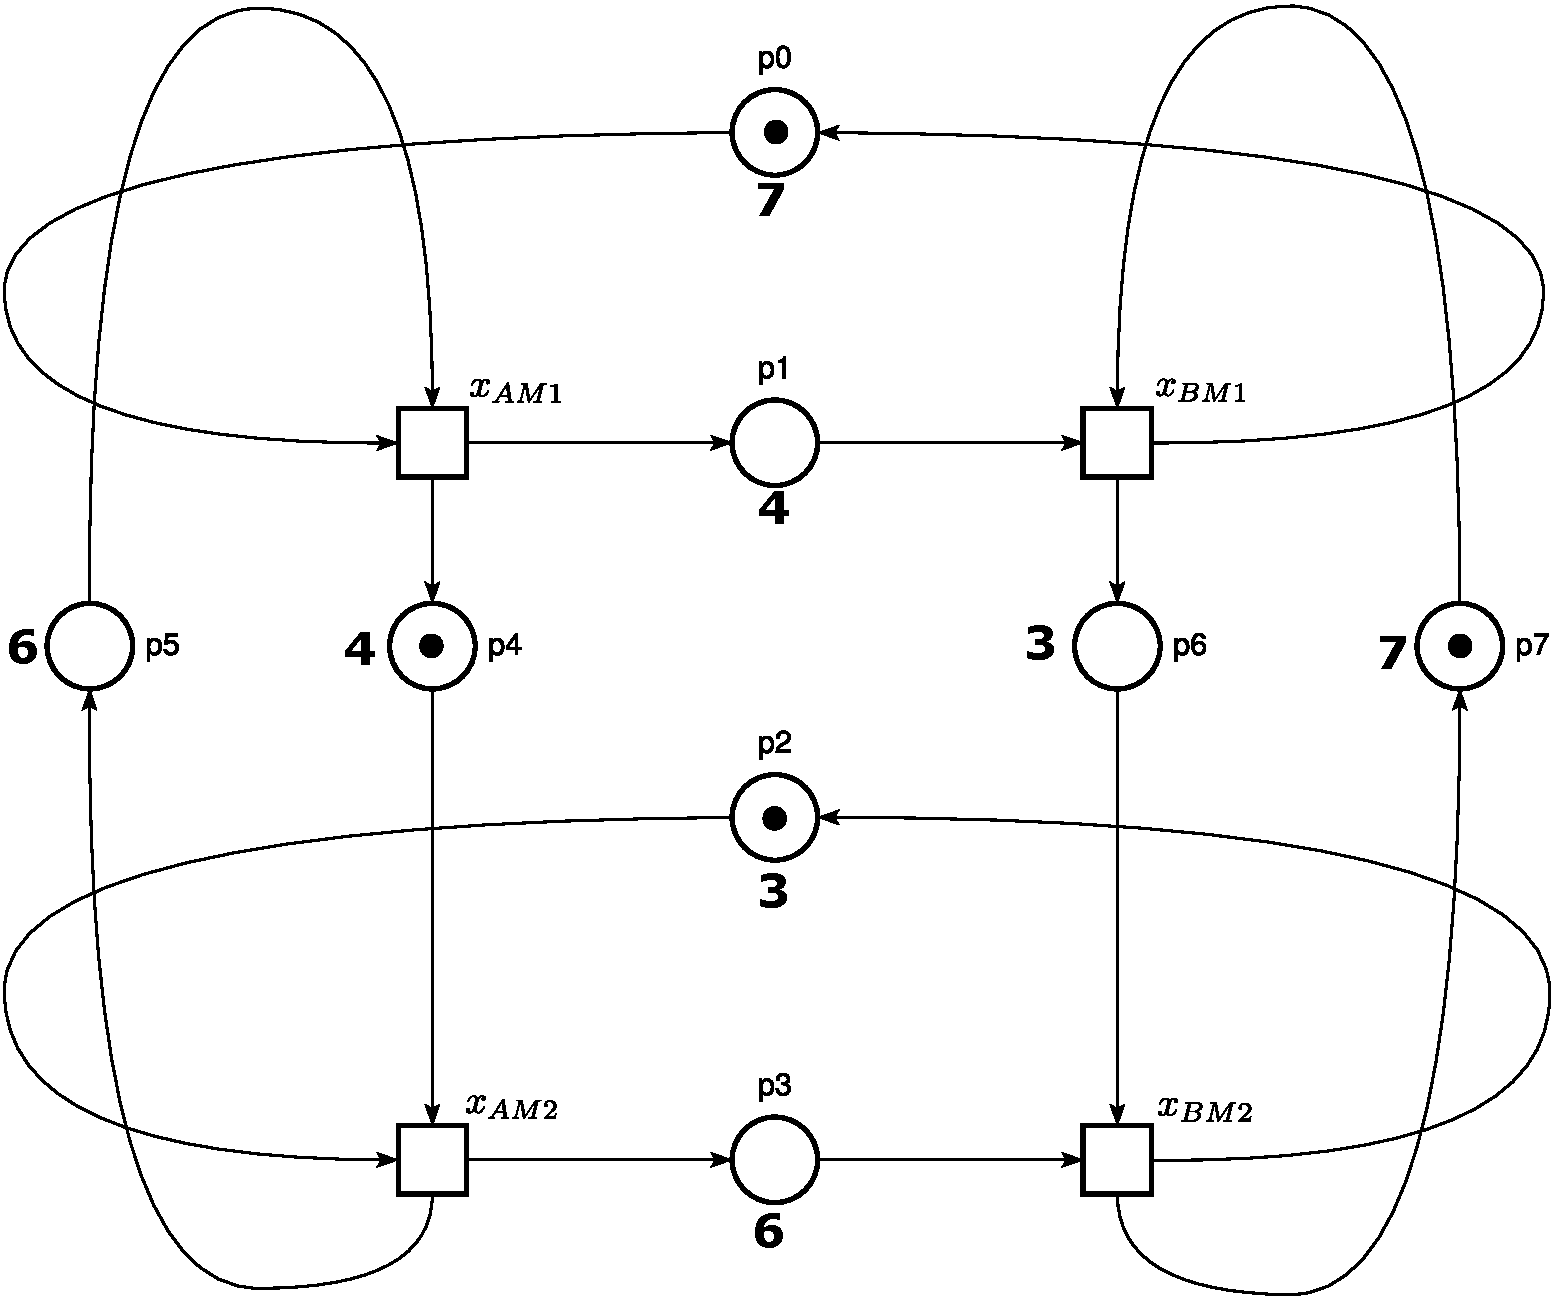
\includegraphics[width = \textwidth]{./II/images/GET_1.pdf}
\caption{\label{fig:get} Graphe des Événements Temporisé de l'ordonnancement 4(\ref{item:o4})}
\end{figure}
\begin{align*}%\label{equ:ordo4}
\left\lbrace
\begin{array}{lcl}
x_{AM_1}(k)&=& 20x_{AM_1}(k-1) \oplus 19x_{BM_2}(k-1) \oplus 15x_{AM2}(k-1)\\
x_{AM_2}(k)&=& 14x_{AM_1}(k-1) \oplus 13x_{BM_2}(k-1) \oplus  9x_{AM2}(k-1)\\
x_{BM_1}(k)&=&  4x_{AM_1}(k-1) \oplus  3x_{BM_2}(k-1)\\
x_{BM_2}(k)&=& 10x_{BM_2}(k-1) \oplus 11x_{AM_1}(k-1) \oplus  6x_{AM2}(k-1)\\
\end{array}
\right.
\end{align*}
\begin{align}\label{eqn::ee_Ordo4}
X(k) = \begin{pmatrix}
20&15&\epsilon&19\\
14&8&\epsilon&13\\
4&\epsilon&\epsilon&3\\
11&6&\epsilon&10
\end{pmatrix}X(k-1) = A_3X(k-1)
\end{align}